\section{Auswertung}
\label{sec:Auswertung}

\subsection{Untergrund}
  Die aufgenommenen Messwerte sind in \autoref{fig:T_I_plot_beide_Messung} zu sehen.
  Der Depolarisationsstrom ist hier in Abhängigkeit von der Temperatur der Probe geplottet worden.
  Der Untergrund wird nun durch eine e-Funktion dargestellt.
  Dafür wird die Funktion
  \begin{equation*}
    f(T) = a \cdot \exp(\frac{-m}{T})
  \end{equation*}
  an den Anstieg des zweiten Maximums gefittet.
  Dabei ergeben sich folgende Werte:
  \begin{align*}
    &\text{Messung 1}\\
    &a =  4694721532.15 \pm 2346550842.93 &&  m = 5899.27 \pm 150.55 \, ,\\
    &\text{Messung 2}\\
    &a = 903022970.16 \pm 484903733.29 &&  m = 5359.79 \pm 165.24 \, .\\
  \end{align*}
  In \autoref{fig:T_I_plot_Untergrund} sind die entsprechenden Untergrund-Fits zu sehen.

\begin{figure}
  \centering
  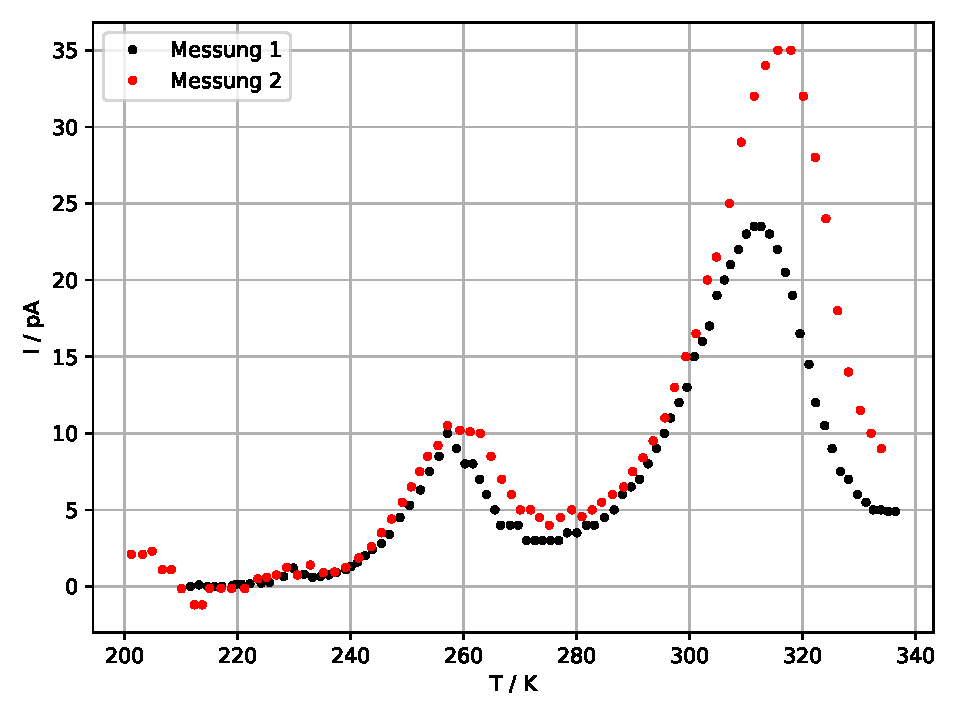
\includegraphics[width = 0.7\textwidth]{build/plot.pdf}
  \caption{Die aufgenommenen Messwerte. Bei Messung 1 wird eine Heizrate von $b = \SI{1.5}{\celsius\per\minute}$ erzielt, 
  bei Messung 2 soll $b = \SI{2}{\celsius\per\minute}$ betragen.}
  \label{fig:T_I_plot_beide_Messung}
\end{figure} % OK, Heizrate mit Kelvin angeben ?

\begin{figure}
  \begin{subfigure}[b]{.5\linewidth}
    \centering
    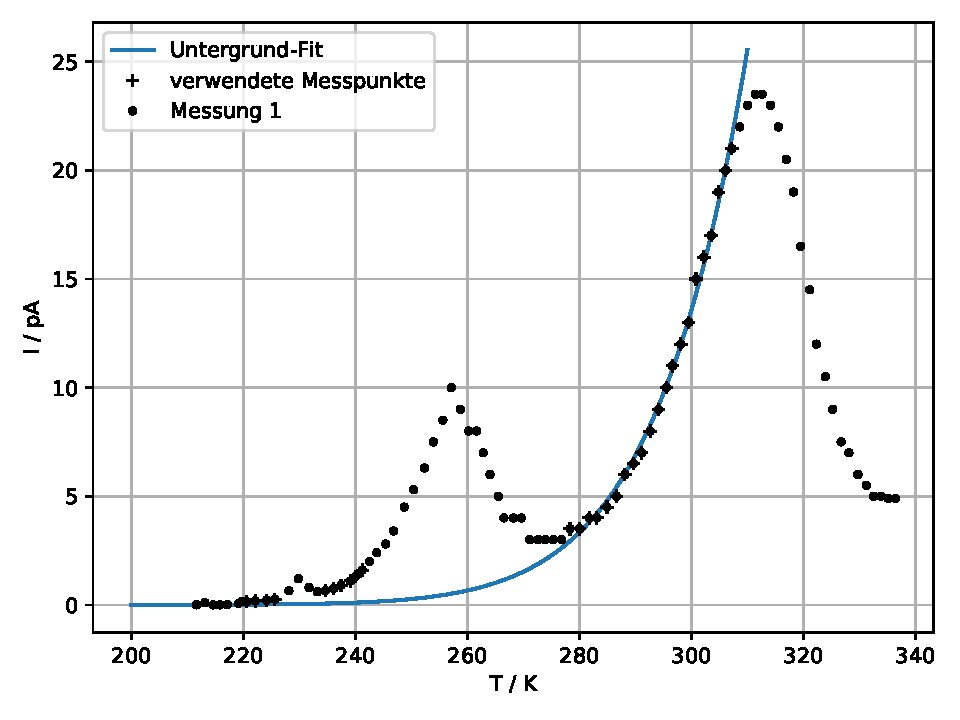
\includegraphics[height=5cm, keepaspectratio]{build/untergrund_1.pdf}
  \end{subfigure}
  
  \begin{subfigure}[b]{.5\linewidth}
    \centering
    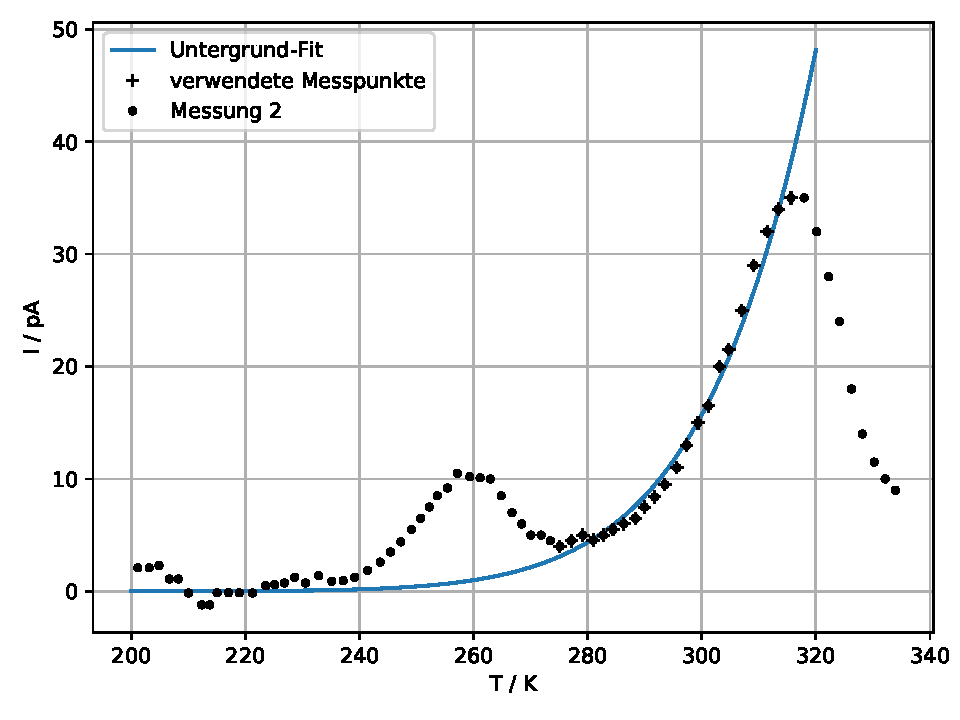
\includegraphics[height=5cm, keepaspectratio]{build/untergrund_2.pdf}
  \end{subfigure}
  
  \caption{Die gefittete Untergrundfunktion mit der Form einer e-Funktion.
    Die Messwerte, die den Anstieg des zweiten Maximums bilden, werden für den Fit verwendet.}
  \label{fig:T_I_plot_Untergrund}
\end{figure} % OK

\subsection{Heizrate}
  Die aufgenommenen Messwerte können auch in ein Zeit-Temperatur Diagramm dargestellt werden.
  Dieses ist in \autoref{fig:t_T_plot} zu sehen.
  Um die Heizrate der jeweiligen Messung zu bestimmen, wird eine lineare Ausgleichsrechnung durhgeführt.
  Die zu fittende Funktion hat die Form
  \begin{equation*}
    T(t) = b * t + T_0 \, .
  \end{equation*}
  Es ergibt sich für die erste Messung:
  \begin{align*}
    b = (1.46 \pm 0.0037) \si{\kelvin\per\minute} &&  T_0 = 210.92 \pm 0.1885\\
  \end{align*}
  und für die zweite Messung:
  \begin{align*}
    b =  1.87 \pm 0.0049  &&  T_0 = 198.95 \pm  0.2027 \, . \\
  \end{align*}
  Die beiden Messungen sowie ihre jeweiligen Ausgleichsgeraden sind in \autoref{fig:t_T_plot_1_Ausgleich} und \autoref{fig:t_T_plot_2_Ausgleich} zu sehen.

  \begin{figure}
    \centering
    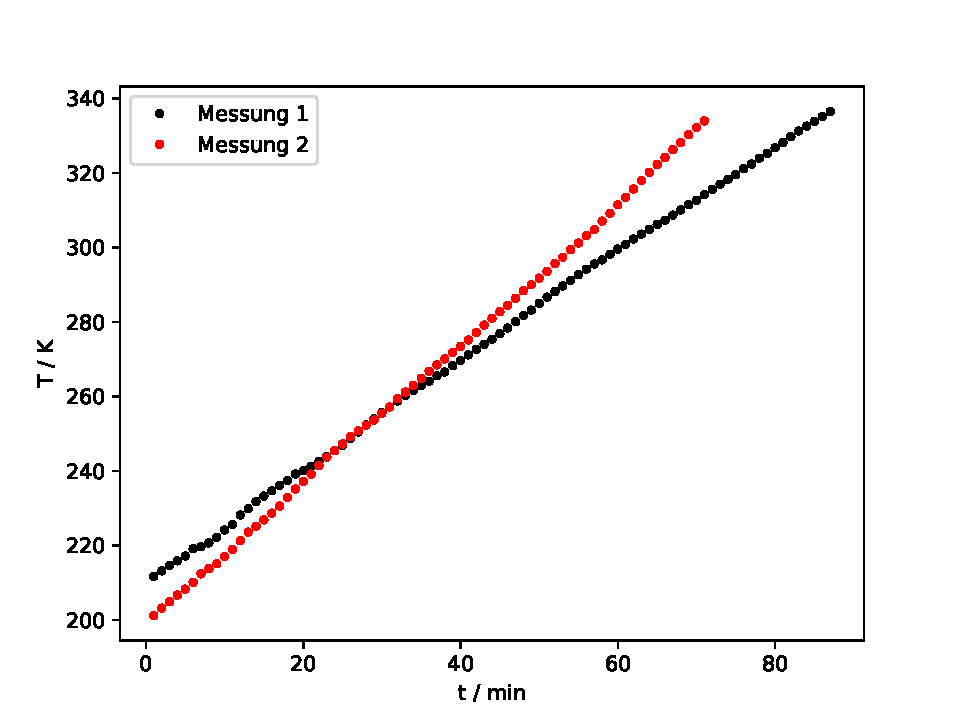
\includegraphics[width = 0.7\textwidth]{build/zeit_temp.pdf}
    \caption{Die aufgenommenen Messwerte. Bei Messung 1 wird eine Heizrate von $b = \SI{1.5}{\celsius\per\minute}$ erzielt, 
    bei Messung 2 soll $b = \SI{2}{\celsius\per\minute}$ betragen.}
    \label{fig:t_T_plot}
  \end{figure} % OK, eig könnte man beschreibung so lassen bzw. wat soll man sonst da schreiben

  \begin{figure}
    \begin{subfigure}[b]{.5\linewidth}
      \centering
      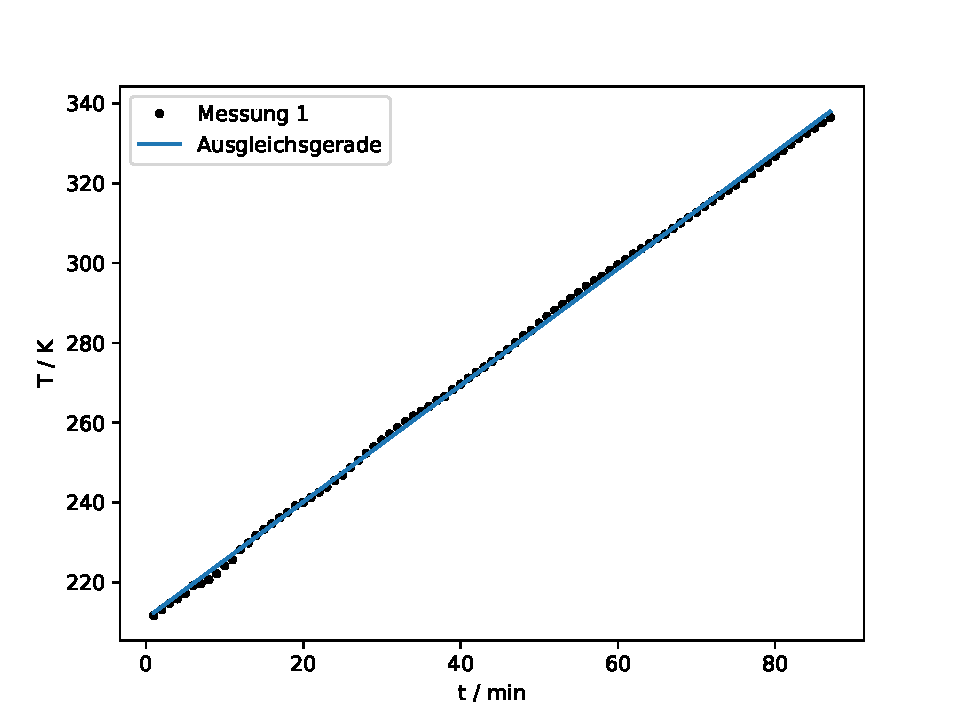
\includegraphics[height=5cm, keepaspectratio]{build/zeit_temp_fit_1.pdf}
      \caption{Durch den Fit ergibt sich für $b = \SI{}{\celsius\per\minute}$.}
    \label{fig:t_T_plot_1_Ausgleich}
    \end{subfigure}
    \begin{subfigure}[b]{.5\linewidth}
      \centering
      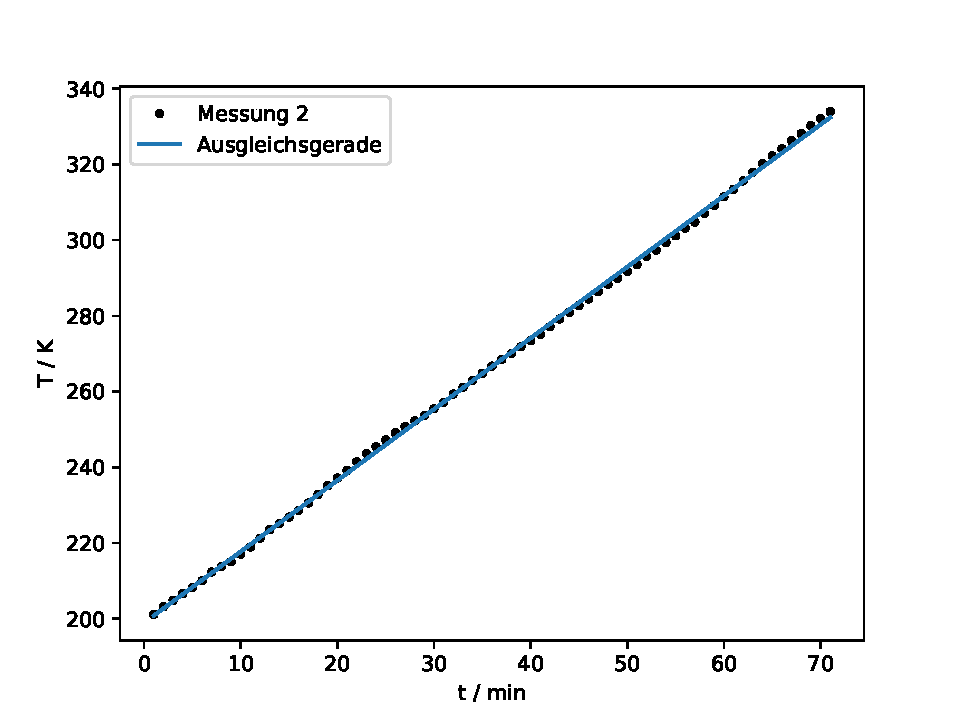
\includegraphics[height=5cm, keepaspectratio]{build/zeit_temp_fit_2.pdf}
      \caption{Durch den Fit ergibt sich für $b = \SI{}{\celsius\per\minute}$.}
    \label{fig:t_T_plot_2_Ausgleich} 
    \end{subfigure}
    \caption{Die aufgenommenen Messwerte der Messungen und der dazugehörige Fit um die Heizrate zu bestimmen.}
  \end{figure} % OK, vielleicht auch ermittelte Heizrate hier rein schreiben?

\subsection{Aktivierungsenergie - Erste Methode}
  Zur Bestimmung der Aktivierungsenergie mithilfe des Maximums werden die Messwerte zunächst in eine andere Darstellung gebracht.
  Nach THEORIE wird der Logarithmus des Depolarisationsstrom gebildet und gegen die inverse Temperatur abgebildet.
  Die jeweiligen Diagramme sind in \autoref{fig:log_I_1_durch_T_Messung_1} und \autoref{fig:log_I_1_durch_T_Messung 2} zu finden.
  Mithilfe von THEORIE wird eine Ausgleichsrechnung durchgeführt.
  Die zu fittende Funktion hat dabei die Form
  \begin{equation*}
    \ln{I(T)} = c - m \cdot \frac{1}{T} \, .
  \end{equation*}
  Die ermittelten Werte sind für Messung 1:
  \begin{align*}
    c =  31.97 \pm  0.62 && m = -7618.67 \pm 150.70  \,  \\
  \end{align*}
  und für Messung 2:
  \begin{align*}
    c = 22.97 \pm  1.84 && m = -5348.16 \pm 444.14  \, . \\
  \end{align*}
  Die Ausgleichsgeraden sind ebenfalls in \autoref{fig:log_I_1_durch_T_Messung_1} und \autoref{fig:log_I_1_durch_T_Messung 2} zu finden.

  \begin{figure}
    \begin{subfigure}[b]{.5\linewidth}
      \centering
      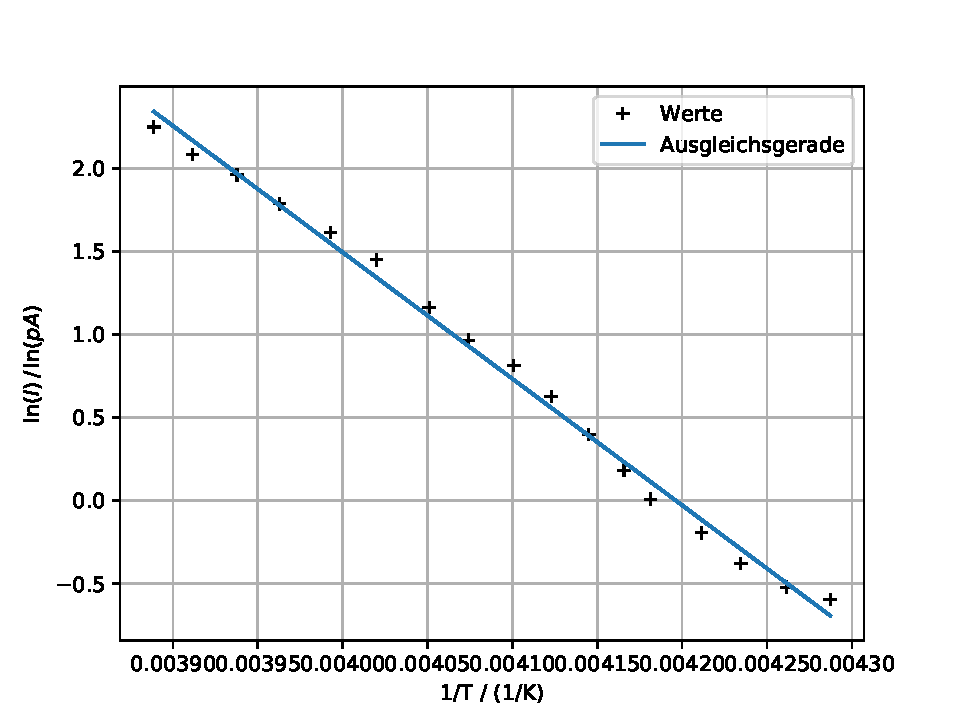
\includegraphics[height=5cm, keepaspectratio]{build/log(I)_1durchT_1.pdf}
      \caption{$\log{I} gegen \frac{1}{T}$ aufgetragen.}
      \label{fig:log_I_1_durch_T_Messung_1}
    \end{subfigure}

    \begin{subfigure}[b]{.5\linewidth}
      \centering
      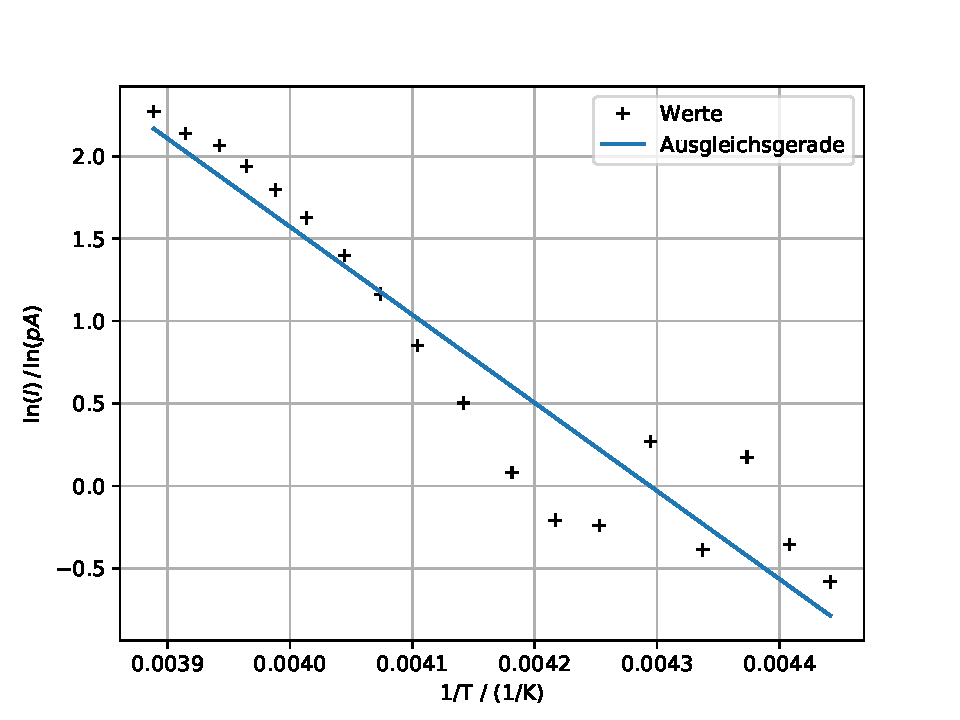
\includegraphics[height=5cm, keepaspectratio]{build/log(I)_1durchT_2.pdf}
      \caption{was sagt uns das? genau. gar nichts}
      \label{fig:log_I_1_durch_T_Messung 2}
    \end{subfigure}
    \caption{Korrigierte Messwerte, nur erster Peak, Ausgleichsrechnung}
  \end{figure} % Ok, Beschreibung?

  \noindent
  Aus THEORIE ergibt sich dann für die jeweilige Aktivierungsenergie $W$
  \begin{align*}
    W   &= -k_\text{B} \cdot m \\
    \implies W_{1,1} &= (1.052 \pm 0.021) \cdot 10^{-19} \si{\joule} &= (0.657 \pm 0.013) \, \si{\electronvolt} \, , \\
    \implies W_{1,2} &= (7.4 \pm 0.6) \cdot 10^{-20} \si{\joule} &= (0.657 \pm 0.013) \, \si{\electronvolt}  \, .\\
  \end{align*}

\subsection{Aktivierungsenergie - Zweite Methode}
  Der korrigierte Stromverlauf wird nun betrachtet.
  Dieser ist für beide Messungen in \autoref{fig:I_T_korrigiert} zu finden.

  \begin{figure}
    \begin{subfigure}[b]{.5\linewidth}
      \centering
      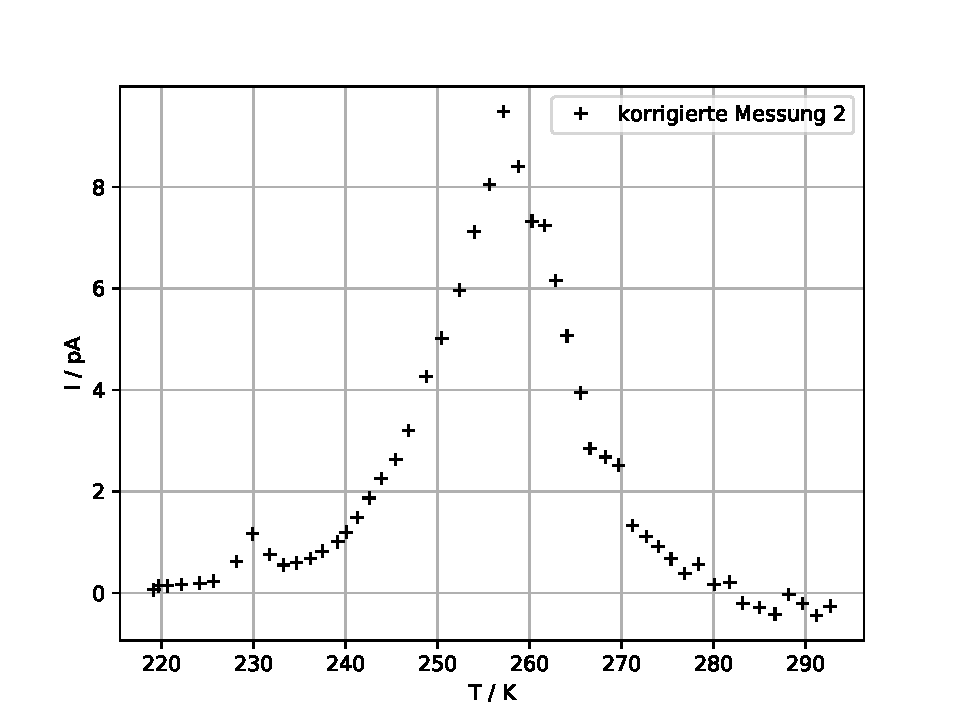
\includegraphics[height=5cm, keepaspectratio]{build/korrigierte_werte_1.pdf}
    \end{subfigure}

    \begin{subfigure}[b]{.5\linewidth}
      \centering
      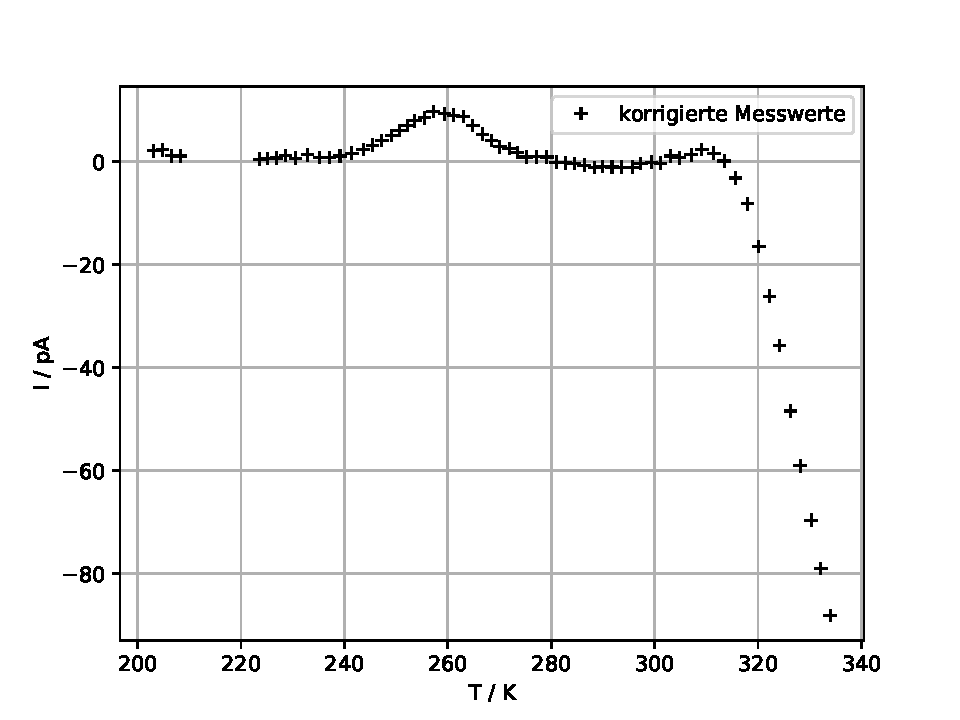
\includegraphics[height=5cm, keepaspectratio]{build/korrigierte_werte_2.pdf}
    \end{subfigure}

    \caption{Die korrigierten Messwerte der jeweiligen Messung.}
    \label{fig:I_T_korrigiert}
  \end{figure} % OK idk

  \noindent
  Zusätzlich wird nur der Peak der jeweiligen Messung betrachtet.
  Nach THEORIE wird $\frac{1}{T}$ gegen $ln ()$ aufgenommen um dadurch eine lineare Ausgleichsrechnung der Form
  \begin{equation*}
    y = m \cdot x + b 
  \end{equation*}
  durchzuführen.
  Die Diagramme mit den dazugehörigen Ausgleichsgeraden sind in \autoref{fig:Trapez} zu finden.
  Die ermittelten Werte betragen:
  \begin{align*}
    &\text{Messung 1} \\
    &m = 9541.25 \pm 135.01 && b= -34.97 \pm  \, 0.54 , \\ 
    &\text{Messung 2} \\
    &m = 10269.27 \pm 133.28 && b = -37.83 \pm 0.53\, . \\
  \end{align*}
  \noindent
  Mithilfe von THEORIE wird die Aktivierungsenergie $W$ und die Relaxationszeit $\tau$ bestimmt.
  Es folgt:
  \begin{align*}
    W_{2,1} &= (1.317 \pm 0.019) \cdot 10^{-19} \, \si{\joule} &= (0.822 \pm 0.012) \, \si{\electronvolt} \, ,\\
    W_{2,2} &= (1.418 \pm 0.018) \cdot 10^{-19} \, \si{\joule} &= (0.885 \pm 0.011) \, \si{\electronvolt} \, .\\
  \end{align*}

  \begin{figure}
    \begin{subfigure}[b]{.5\linewidth}
      \centering
      \includegraphics[height=5cm, keepaspectratio]{build_j/log()_2durchT_1.pdf}
      \caption{Messung 1}
    \end{subfigure}

    \begin{subfigure}[b]{.5\linewidth}
      \centering
      \includegraphics[height=5cm, keepaspectratio]{build_j/log()_2durchT_2.pdf}
      \caption{Messung 2}
    \end{subfigure}

    \caption{Messwerte der Messungen und die jeweiligen Fits.}
    \label{fig:Trapez}
  \end{figure} % OK Beschreibbung

\subsection{Relaxationszeit}
  Mit den ermittelten Heizraten und Aktivierungsenergien kann nach THEORIE die Relaxationszeit bestimmt werden.
  Die Heizrate für Messung 1 beträgt $b_1 = $ und für Messung 2 $b_2 = $.
  Somit folgt für die jeweilige Relaxationszeit $\tau$ mit den Aktivierungsenergien $W$ aus der ersten Methode:
  \begin{align*}
    \tau_{1,1} = -0.00167 \pm 0.00007 &&  \tau_{1,2} = -0.0034 \pm 0.0006 \, . \\
  \end{align*}
  Dabei wurde für $T_\text{max,1} = \SI{38.3}{\celsius} = \SI{311.45}{\kelvin} $ und $T_\text{max,2} = \SI{42.5}{\celsius} = \SI{315.65}{\kelvin}$ ermittelt.
  Bei dieser Temperatur wurde der maximale Depolarisationsstrom beobachtet.

  \noindent
  Mithilfe der zweiten Methode wird die Relaxationszeit auch mit THEORIE bestimmt.
  Es folgt für die jeweilige Messung:
  \begin{align*}
    \tau_{2,1} =  0.001066 \pm 0.000030 &&  \tau_{2,2} = 0.000920 \pm 0.000024\, . \\
  \end{align*}
